% APA 7 student paper - Custom Vision: Animal Identification.
\documentclass[a4paper,12pt]{article}
\usepackage[T1]{fontenc}
\usepackage[spanish]{babel}
\usepackage{lmodern}
\usepackage{setspace}
\usepackage[a4paper,top=2.54cm,bottom=2.54cm,left=2.54cm,right=2.54cm,
  headheight=14pt]{geometry}
\usepackage{indentfirst}
\usepackage{booktabs}
\usepackage{float}
\usepackage{graphicx}
\usepackage{caption}
\usepackage{fancyhdr}
\usepackage{titlesec}
\usepackage[hidelinks]{hyperref}
\usepackage{apacite}

\doublespacing
\setlength{\parindent}{1.27cm}
\setlength{\emergencystretch}{2em}

\titleformat{\section}{\normalfont\bfseries\centering}{}{0pt}{}
\titleformat{\subsection}{\normalfont\bfseries}{}{0pt}{}
\titleformat{\subsubsection}{\normalfont\bfseries\itshape}{}{0pt}{}

\floatstyle{plaintop}\restylefloat{figure}
\captionsetup{position=top,labelsep=newline,labelfont=bf,textfont=it,
  justification=raggedright,singlelinecheck=false,skip=4pt}
\AtBeginDocument{\iflanguage{spanish}{\captionsetup[table]{name=Tabla}}{}}

\pagestyle{fancy}
\fancyhf{}
\rhead{\thepage}
\renewcommand{\headrulewidth}{0pt}

\renewcommand{\doiprefix}{https://doi.org/\ignorespaces}

\AtBeginDocument{%
  \renewcommand{\BOthers}{et al}%
  \renewcommand{\BOthersPeriod}{et al.}%
  \renewcommand{\BRetrievedFrom}{}%
  \renewcommand{\BRetrieved}[1]{}%
}

\begin{document}

  \begin{center}
    \vspace*{2cm}
    \textbf{Custom Vision: Identificaci\'on de Animales con Azure AI Services}
    \vspace{\baselineskip}

    Jheison Martinez Bolivar

    \vspace{\baselineskip}
    Maestr\'ia en Inteligencia Artificial, Universidad de La Salle

    Aprendizaje de M\'aquina

    jhmartinez07@unisalle.edu.co

    Noviembre 2026
  \end{center}
  \newpage

  \begin{abstract}
    Se construy\'o un clasificador de im\'agenes de elefantes, jirafas y leones con Azure Custom Vision \cite{microsoft_customvision2024} sobre Azure AI Services \cite{microsoft_cognitiveservices2024}. La suscripci\'on Azure for Students impone la policy \textit{sys.regionrestriction} que solo permite \textit{francecentral, belgiumcentral, northcentralus, spaincentral} y \textit{chilecentral}; por ello el instructivo original en \textit{East US} falla con \textit{InvalidTemplateDeployment / RequestDisallowedByAzure}. Verificado por CLI, solo \textit{northcentralus} soporta \textit{CustomVision.Training} y \textit{Prediction}, as\'i que los recursos \textit{labunisalle} y \textit{labunisalle-Prediction} se crearon all\'i en SKU S0. El proyecto \textit{Animal Identification} (Classification, Multiclass, dominio General [A2]) se entren\'o con 17 im\'agenes por clase y Quick Training: Precision, Recall y AP en 100\% sobre entrenamiento. Con 6 im\'agenes nuevas de Wikimedia Commons el modelo publicado acierta 6/6 con confianza media de 96.7\%, con el caso m\'as d\'ebil en una imagen con tres jirafas juntas (87.0\%).
  \end{abstract}

  \section{Recursos en Azure}

  El grupo \textit{lab} ya exist\'ia en \textit{eastus}. El intento del instructivo en \textit{East US} fue bloqueado por la policy de la suscripci\'on. La evidencia por CLI:

  \begin{verbatim}
$ az policy assignment show --name sys.regionrestriction
Allowed: francecentral, belgiumcentral, northcentralus,
  spaincentral, chilecentral
$ az cognitiveservices account list-skus \
  --kind CustomVision.Training --location northcentralus
F0, S0
$ az cognitiveservices account list-skus \
  --kind CustomVision.Training --location francecentral
(vacio)
  \end{verbatim}

  Solo \textit{northcentralus} devuelve SKUs para Training y Prediction; las otras cuatro regiones permitidas devuelven tabla vac\'ia. Se crearon entonces, en el grupo \textit{lab}: \textit{labunisalle} (\textit{CustomVision.Training}, \textit{northcentralus}, S0) y \textit{labunisalle-Prediction} (\textit{CustomVision.Prediction}, \textit{northcentralus}, S0). La Figura 1 muestra la creaci\'on en el portal y la Tabla 1 la verificaci\'on por CLI (\textit{az cognitiveservices account list --resource-group lab}).

  \begin{figure}[H]
    \caption{Creaci\'on de los recursos en el portal de Azure.}
    \label{fig:recursos}
    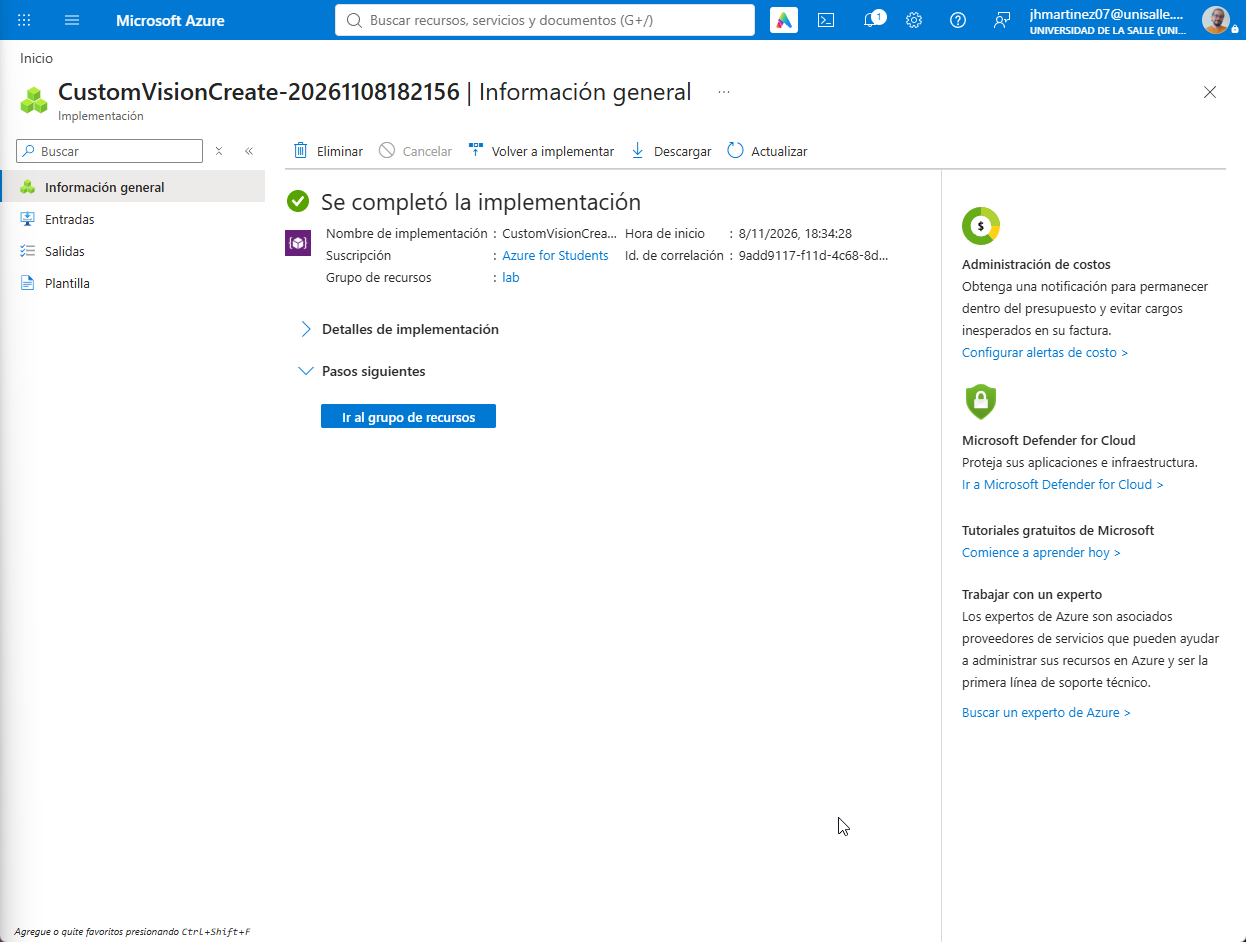
\includegraphics[width=\linewidth]{assets/images/fig_recursos.png}
  \end{figure}

  \begin{table}[H]
    \caption{Recursos verificados por CLI.}
    \label{tab:recursos}
    \begin{tabular}{@{}lll@{}}
      \toprule
      Nombre & Kind & Location / SKU \\
      \midrule
      labunisalle & CustomVision.Training & northcentralus / S0 \\
      labunisalle-Prediction & CustomVision.Prediction & northcentralus / S0 \\
      \bottomrule
    \end{tabular}
    \par\medskip
    \begin{minipage}{\linewidth}
      \footnotesize\textit{Nota.} Salida de \textit{az cognitiveservices account list --resource-group lab}, guardada en \textit{capturas/01-cli-recursos.txt}.
    \end{minipage}
  \end{table}

  \section{Proyecto de Custom Vision}

  El recurso no es el proyecto. El proyecto se crea en \textit{customvision.ai} con el recurso de entrenamiento como contenedor de llaves. Ajustes usados (Figura 2): nombre \textit{Animal Identification}, descripci\'on \textit{Image classification for animals}, recurso \textit{labunisalle [northcentralus]}, tipo Classification, Multiclass (un solo tag por imagen) y dominio General [A2].

  \begin{figure}[H]
    \caption{Creaci\'on del proyecto Animal Identification en customvision.ai.}
    \label{fig:proyecto}
    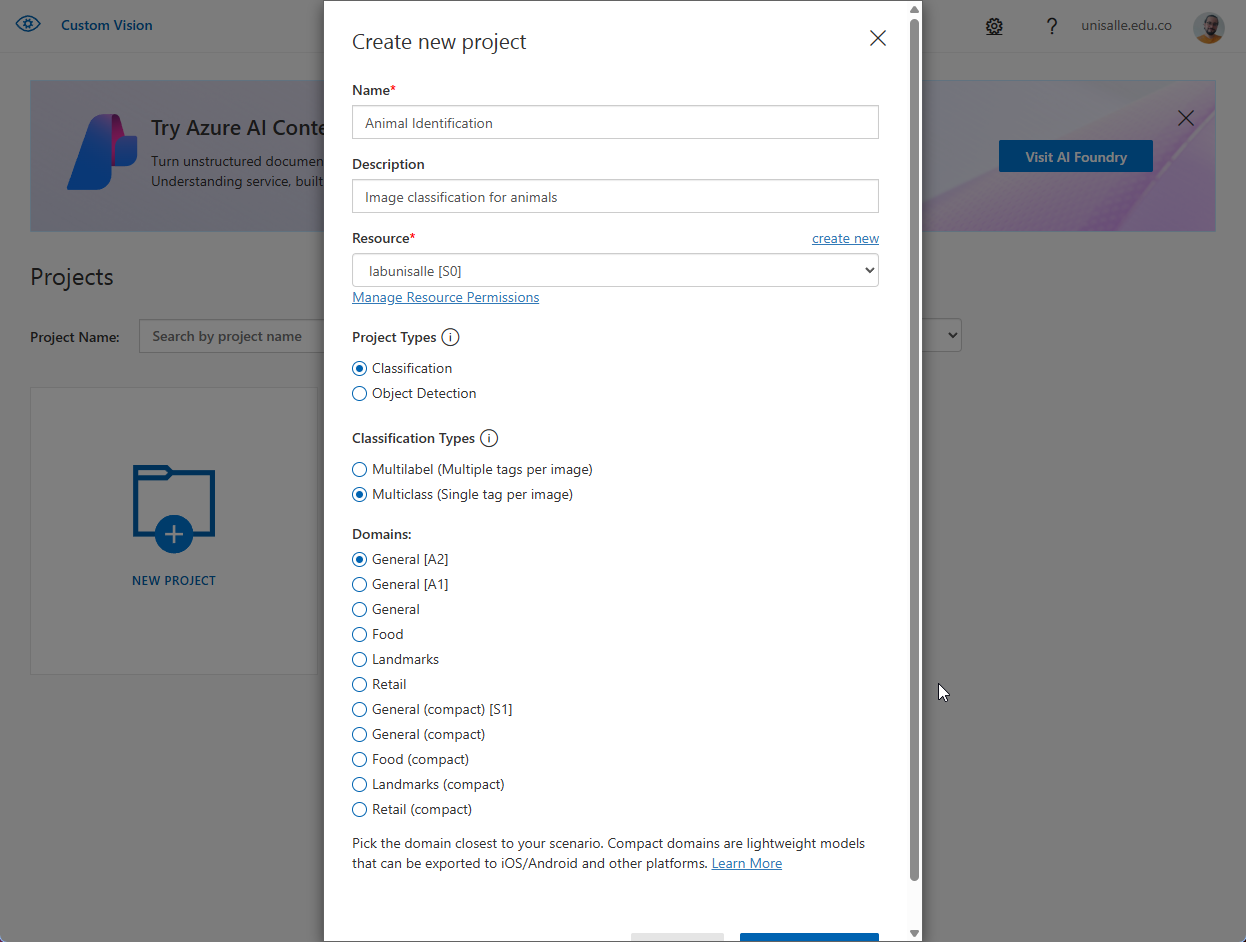
\includegraphics[width=\linewidth]{assets/images/fig_create_project.png}
  \end{figure}

  \section{Carga y Etiquetado}

  Se descarg\'o el paquete de entrenamiento y se subi\'o por etiquetas: \textit{elephant}, \textit{giraffe} y \textit{lion}, con 17 im\'agenes por clase (Figura 3). Cada lote se etiqueta al subirlo; una imagen con m\'as de una etiqueta romper\'ia el supuesto Multiclass, por eso se verifica un solo tag por imagen.

  \begin{figure}[H]
    \caption{Lotes etiquetados por clase, 17 im\'agenes cada uno.}
    \label{fig:tags}
    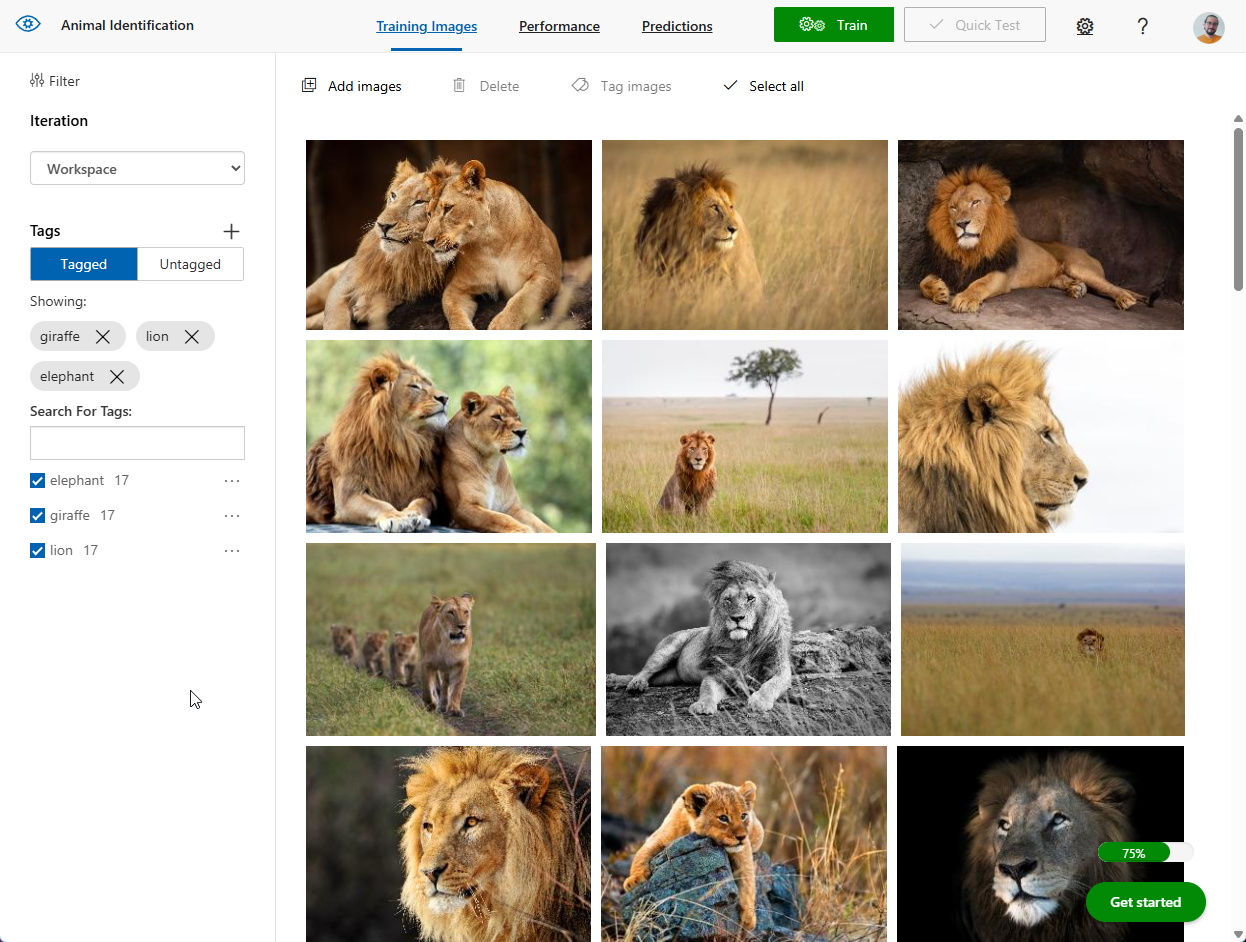
\includegraphics[width=\linewidth]{assets/images/fig_tags.png}
  \end{figure}

  \section{Entrenamiento}

  Se entren\'o con \textit{Train} en modo Quick Training (Figura 4). La Iteraci\'on 1 termin\'o el 8/11/2026 a las 6:51:53 PM con dominio General [A2], ID 71779344-fd60-4c43-9e8f-788ef5230282, tipo Multiclass (Figura 5).

  \begin{figure}[H]
    \caption{Entrenamiento r\'apido lanzado y completado.}
    \label{fig:train}
    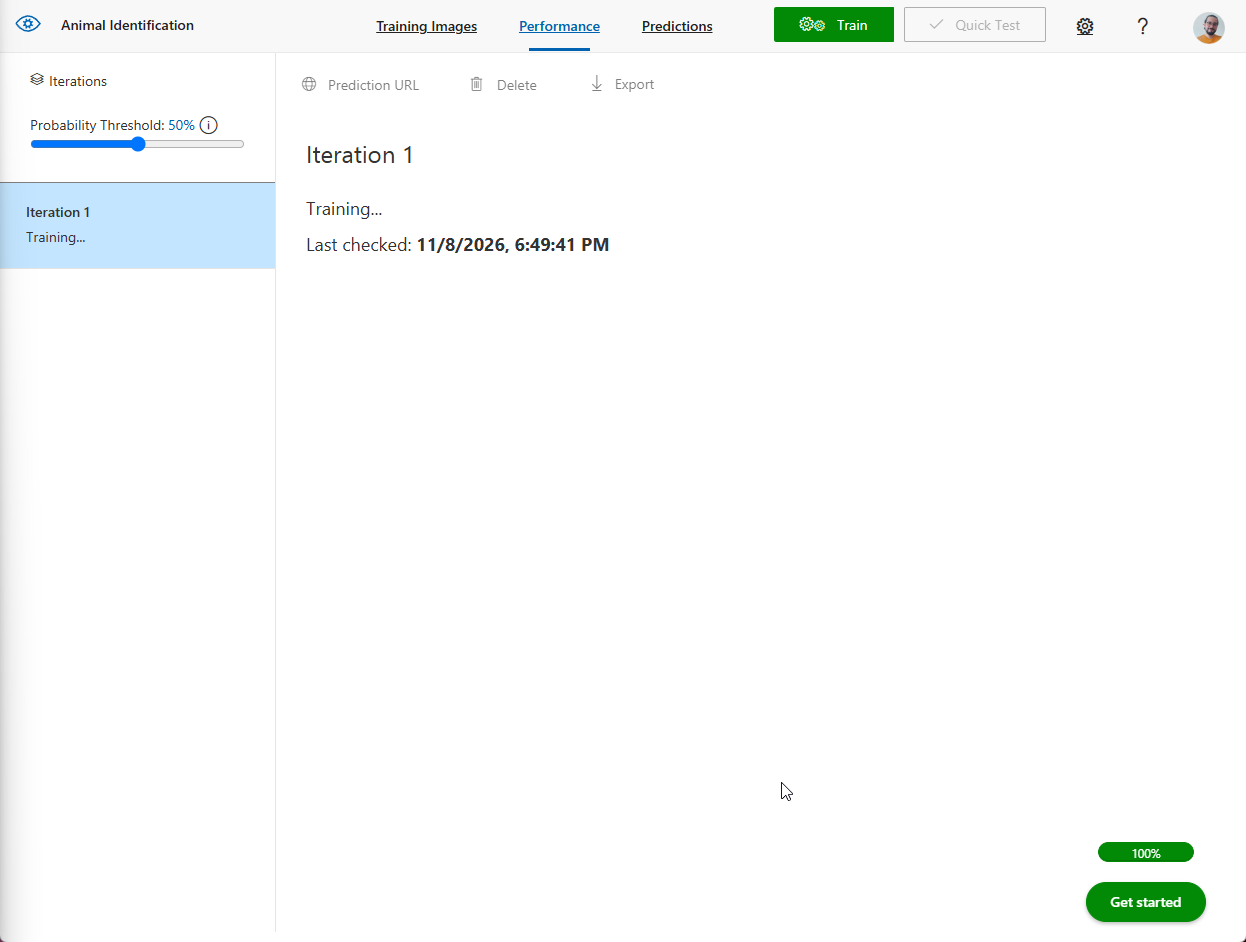
\includegraphics[width=\linewidth]{assets/images/fig_train.png}
  \end{figure}

  \begin{figure}[H]
    \caption{Performance de la Iteraci\'on 1: Precision, Recall y AP globales en 100.0\%.}
    \label{fig:result}
    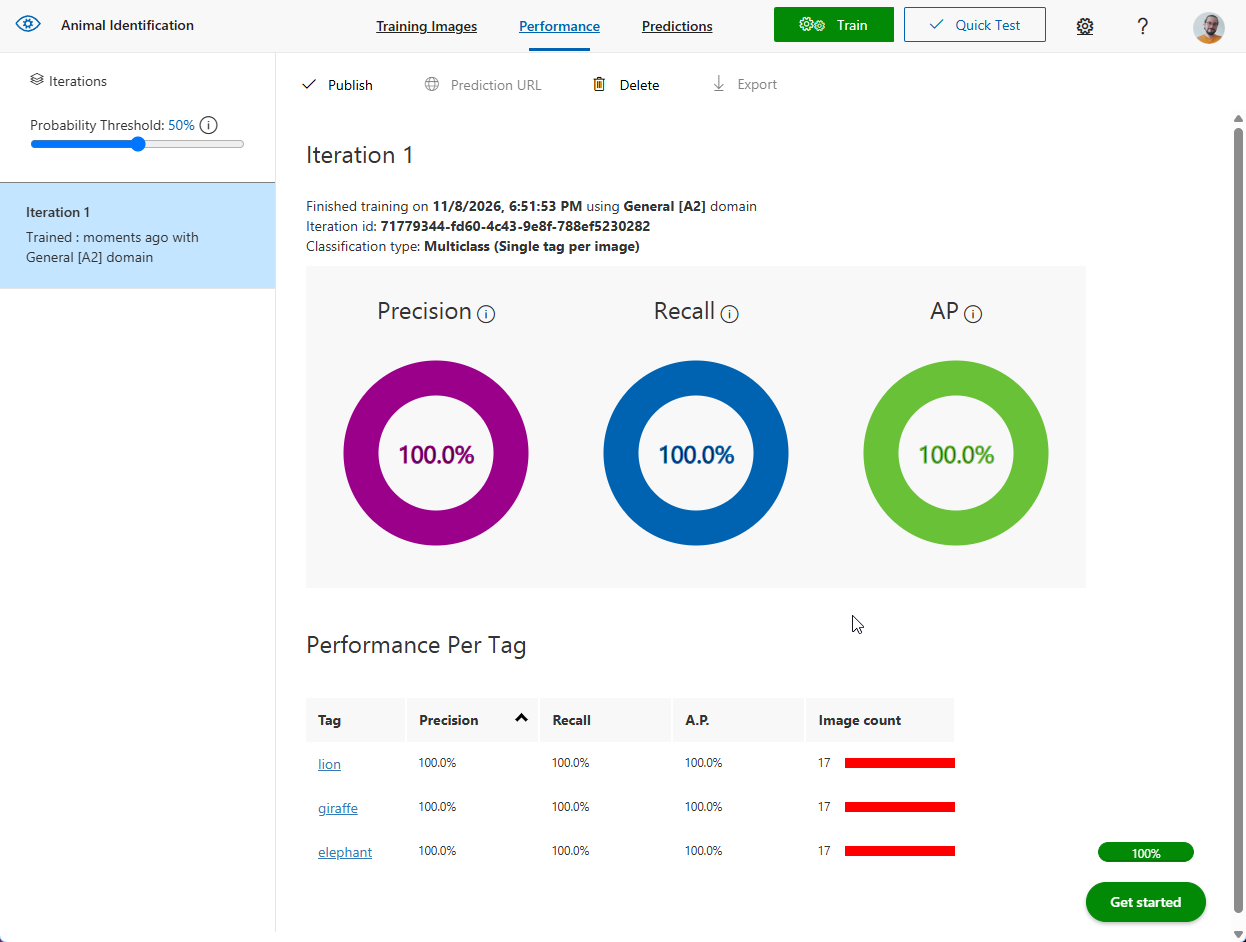
\includegraphics[width=\linewidth]{assets/images/fig_train_result.png}
  \end{figure}

  \section{Evaluaci\'on}

  La Tabla 2 resume el panel Performance con umbral 50\%. El 100\% en las tres m\'etricas y en los tres tags se lee con cautela: con 51 im\'agenes el modelo memoriza el set de entrenamiento; la prueba que importa es con im\'agenes nuevas.

  \begin{table}[H]
    \caption{Performance por tag, Iteraci\'on 1.}
    \label{tab:performance}
    \begin{tabular}{@{}lccc@{}}
      \toprule
      Tag & Precision & Recall & Im\'agenes \\
      \midrule
      lion & 100.0\% & 100.0\% & 17 \\
      giraffe & 100.0\% & 100.0\% & 17 \\
      elephant & 100.0\% & 100.0\% & 17 \\
      \midrule
      Global & 100.0\% & 100.0\% & 51 \\
      \bottomrule
    \end{tabular}
    \par\medskip
    \begin{minipage}{\linewidth}
      \footnotesize\textit{Nota.} Panel Performance de customvision.ai, Iteraci\'on 1, dominio General [A2].
    \end{minipage}
  \end{table}

  Se probaron 6 im\'agenes externas de Wikimedia Commons (carpeta \textit{validacion/}, con fuentes en \textit{FUENTES.txt}), no vistas en entrenamiento, con \textit{Quick Test} sobre la Iteraci\'on 1. La Tabla 3 y las Figuras 6--8 muestran que las 6 clasifican bien, con confianza media de 96.7\%. El caso m\'as d\'ebil es \textit{giraffe\_val\_02} (tres jirafas juntas, 87.0\% con 11.4\% a elephant), el \'unico con oclusi\'on y m\'ultiples instancias.

  \begin{table}[H]
    \caption{Quick Test con im\'agenes nuevas (6/6 aciertos).}
    \label{tab:quicktest}
    \begin{tabular}{@{}lcc@{}}
      \toprule
      Imagen & Predicci\'on correcta & Confianza \\
      \midrule
      elephant\_val\_01 & elephant 98.0\% & 98.0\% \\
      elephant\_val\_02 & elephant 97.6\% & 97.6\% \\
      giraffe\_val\_01 & giraffe 98.5\% & 98.5\% \\
      giraffe\_val\_02 & giraffe 87.0\% & 87.0\% \\
      lion\_val\_01 & lion 99.8\% & 99.8\% \\
      lion\_val\_02 & lion 99.6\% & 99.6\% \\
      \bottomrule
    \end{tabular}
    \par\medskip
    \begin{minipage}{\linewidth}
      \footnotesize\textit{Nota.} Quick Test sobre la Iteraci\'on 1 con im\'agenes de Wikimedia Commons no usadas en entrenamiento.
    \end{minipage}
  \end{table}

  \begin{figure}[H]
    \caption{Quick Test en elefantes nuevos: 98.0\% y 97.6\%.}
    \label{fig:qt1}
    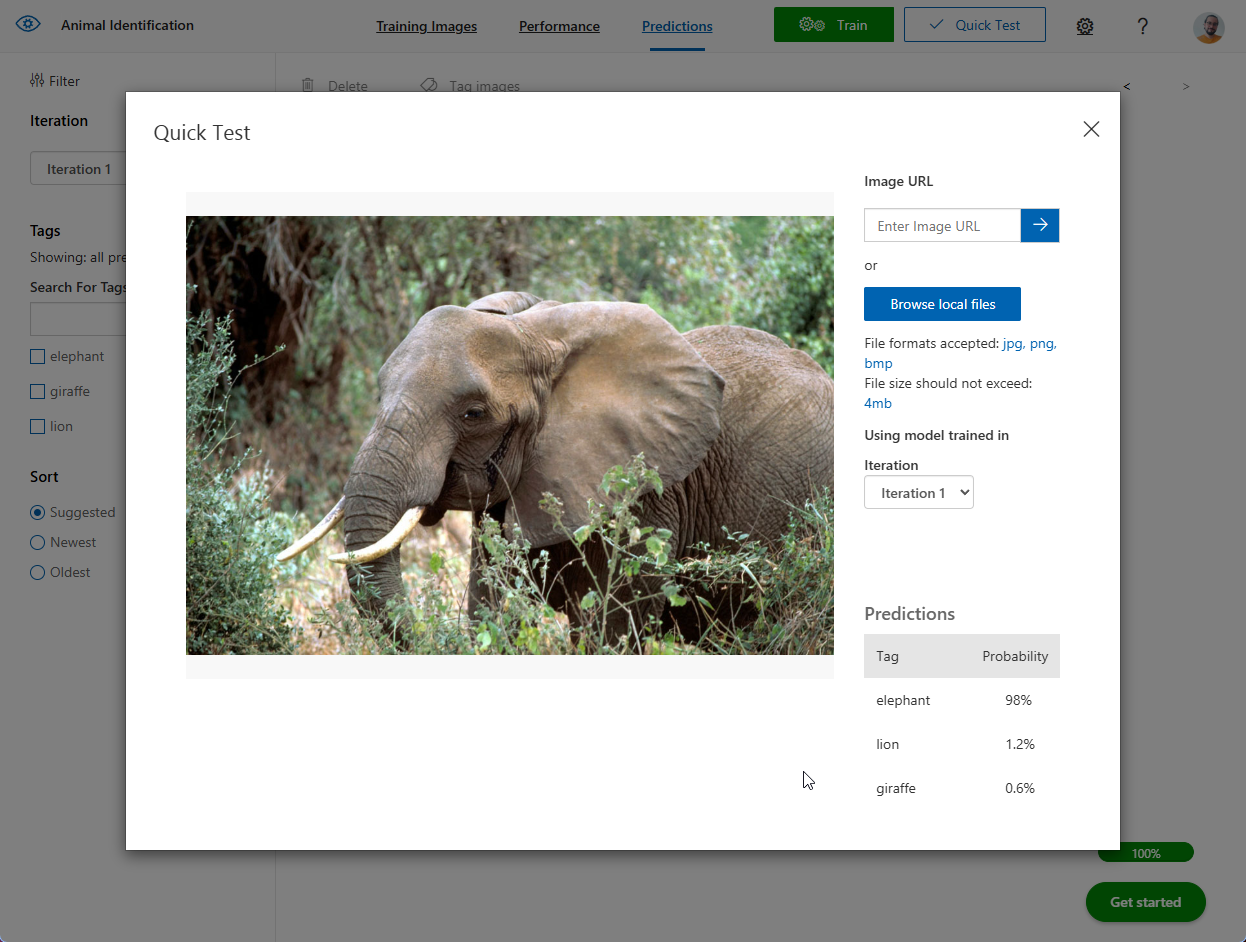
\includegraphics[width=\linewidth]{assets/images/fig_qt_elephant1.png}
    \par\medskip
    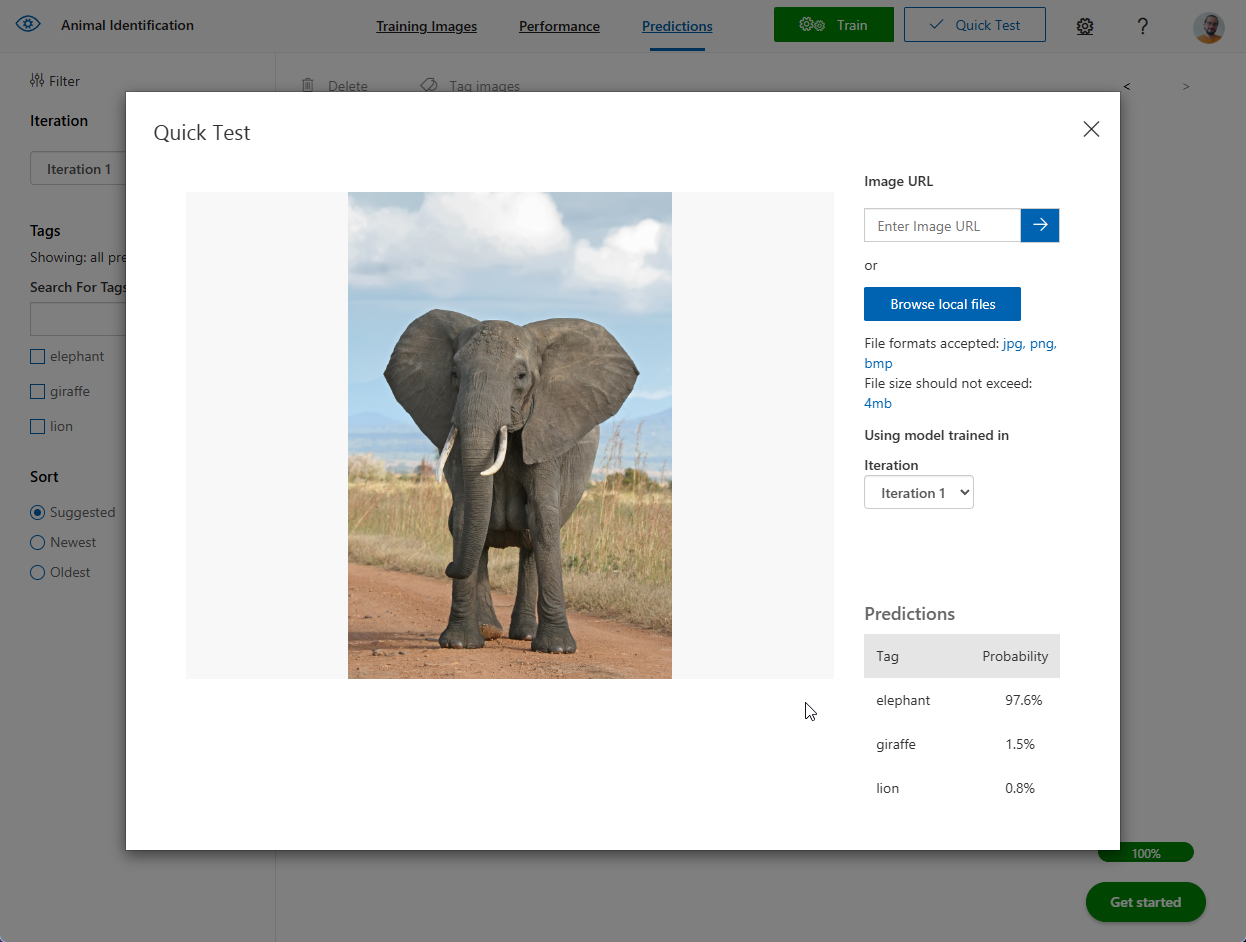
\includegraphics[width=\linewidth]{assets/images/fig_qt_elephant2.png}
  \end{figure}

  \begin{figure}[H]
    \caption{Quick Test en jirafas nuevas: 98.5\% y 87.0\% (tres ejemplares con oclusi\'on).}
    \label{fig:qt2}
    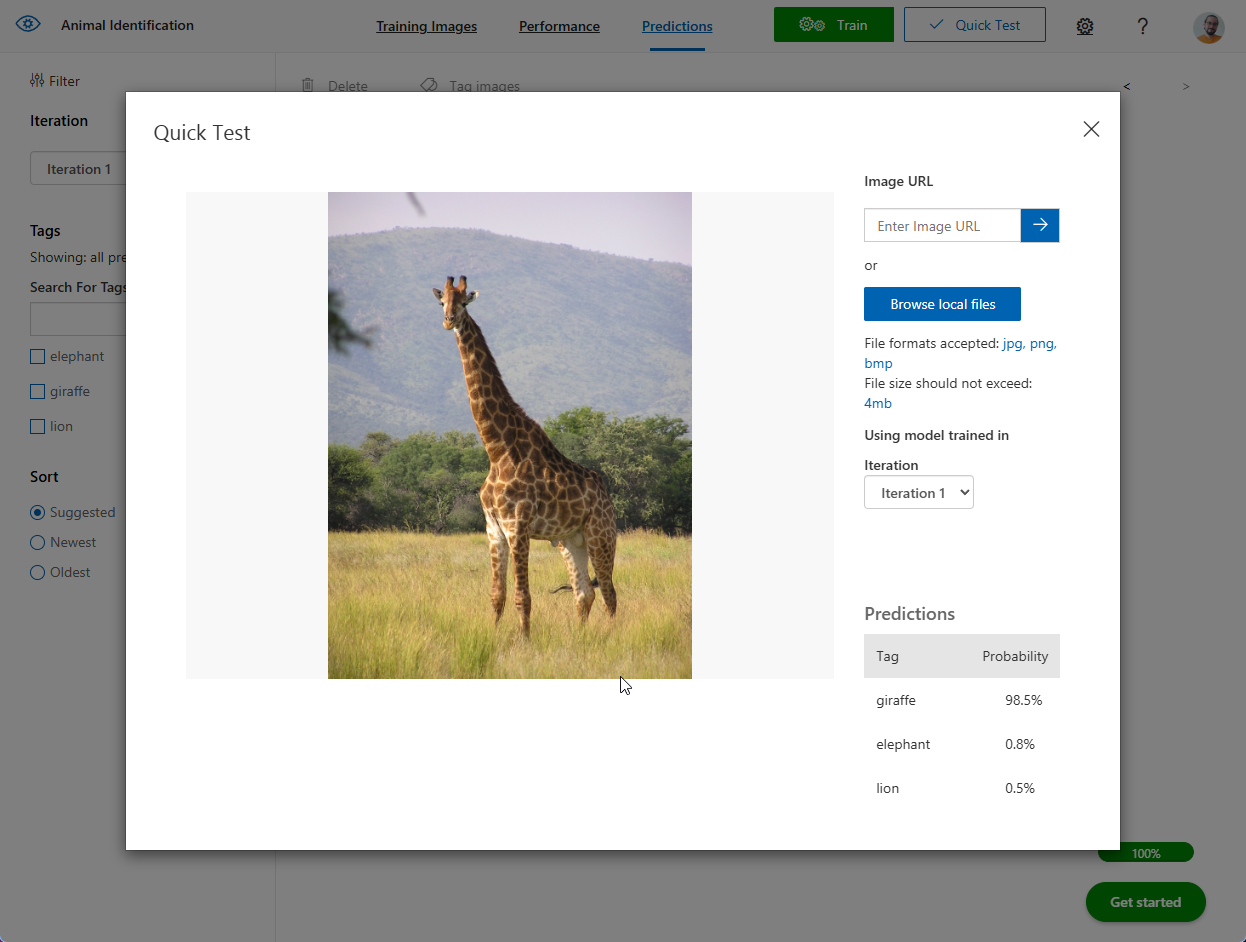
\includegraphics[width=\linewidth]{assets/images/fig_qt_giraffe1.png}
    \par\medskip
    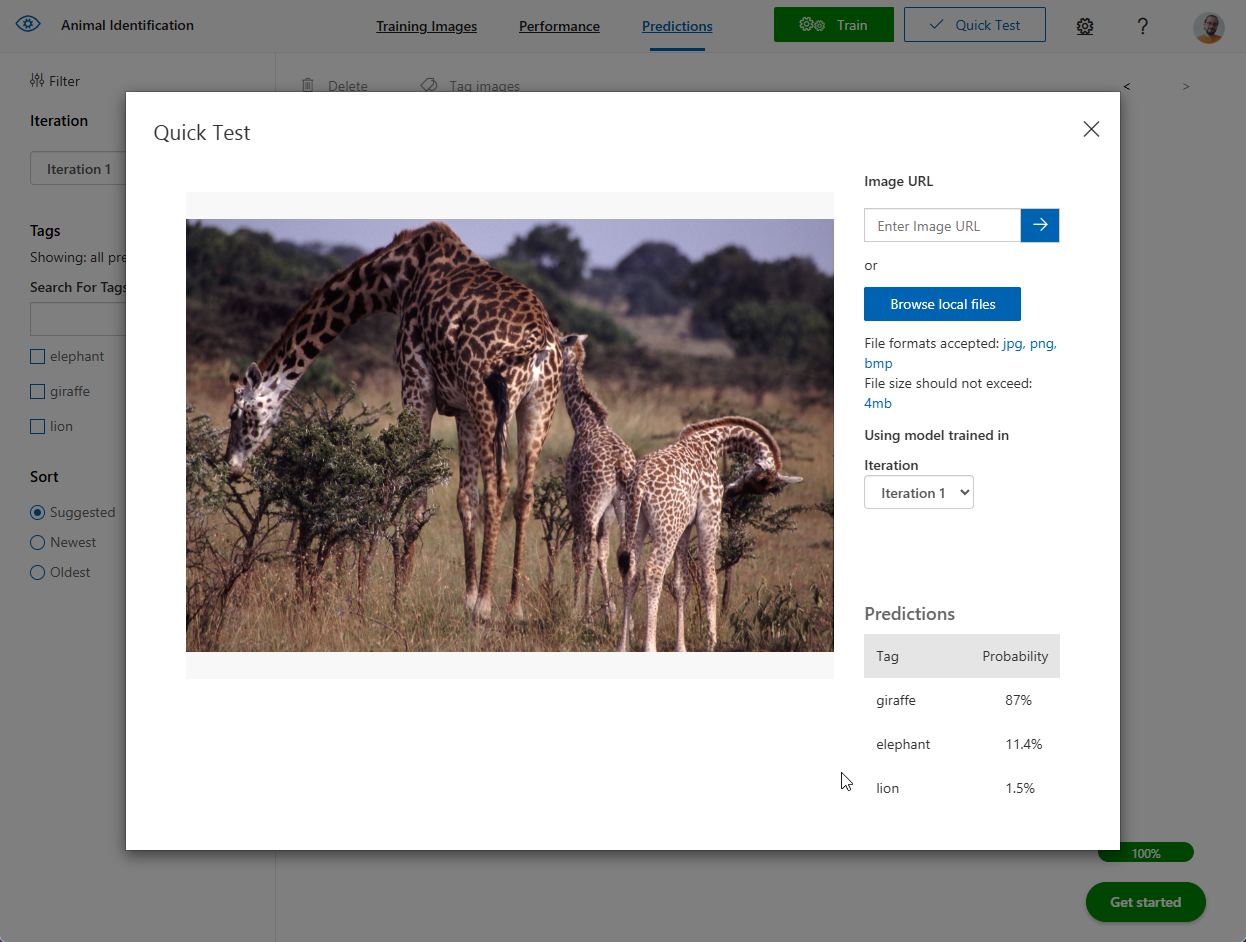
\includegraphics[width=\linewidth]{assets/images/fig_qt_giraffe2.png}
  \end{figure}

  \begin{figure}[H]
    \caption{Quick Test en leones nuevos: 99.8\% y 99.6\%.}
    \label{fig:qt3}
    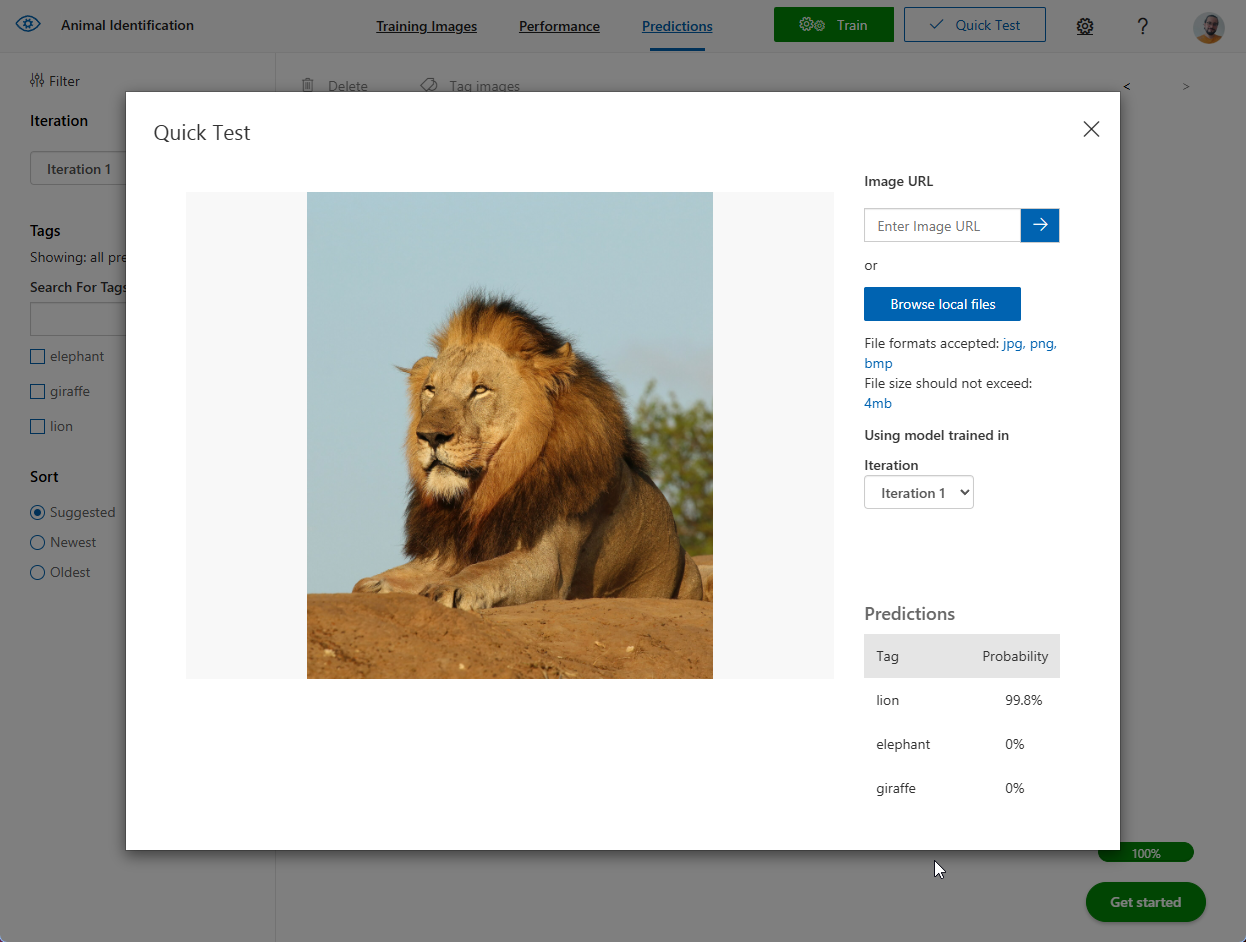
\includegraphics[width=\linewidth]{assets/images/fig_qt_lion1.png}
    \par\medskip
    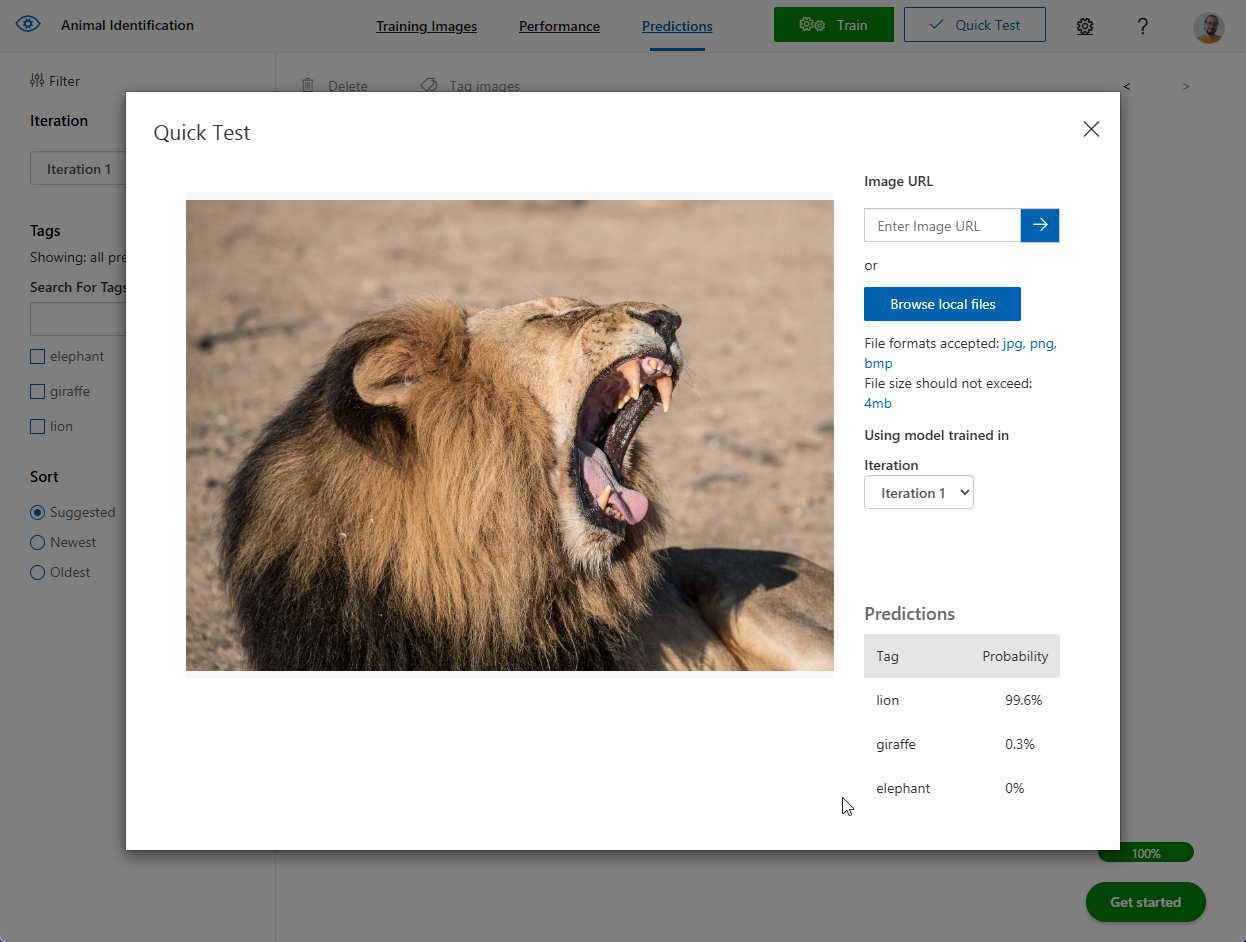
\includegraphics[width=\linewidth]{assets/images/fig_qt_lion2.png}
  \end{figure}

  \section{Publicaci\'on y Cliente}

  La Iteraci\'on 1 se public\'o como modelo \textit{AnimalIdentification-v1} contra el recurso \textit{labunisalle-Prediction} en \textit{northcentralus}. El endpoint de imagen es \textit{https://labunisalle-prediction.cognitiveservices.azure.com/customvision/v3.0/Prediction/8745a5dd-92de-4fd7-967f-642ce3967c6c/classify/iterations/Iteration1/image}, con headers \textit{Prediction-Key: \textless{}clave del portal\textgreater{}} y \textit{Content-Type: application/octet-stream}. La clave completa queda guardada en el portal (\textit{labunisalle-Prediction \textgreater{} Keys and Endpoint}) y no se imprime en este PDF por seguridad; se rota despu\'es de la entrega.

  La prueba del cliente se hizo con \textit{curl} sobre dos im\'agenes de validaci\'on no vistas (salida completa en \textit{capturas/14-cloudshell-test.txt}): \textit{lion\_val\_01.jpg} devuelve lion 0.9986 y \textit{giraffe\_val\_02.jpg} devuelve giraffe 0.8700 con elephant 0.1147. Los valores coinciden con el Quick Test del portal (99.8\% y 87.0\%), as\'i que el modelo publicado responde igual que el evaluado.

  \section{Limitaciones}

  La principal limitaci\'on no es del modelo sino de la suscripci\'on: la policy regional impide seguir literalmente el instructivo en \textit{East US} y obliga a \textit{northcentralus}. El conjunto es peque\~no (51 im\'agenes), as\'i que las m\'etricas describen este ejercicio y no generalizan. El 100\% en entrenamiento confirma memorizaci\'on del set; la evidencia de generalizaci\'on es el 6/6 en im\'agenes nuevas con media de 96.7\%.

  \bibliographystyle{apa7cite}
  \bibliography{bib/references}

\end{document}
